%---------- Quarto Capítulo: Desenvolvimento ----------

\chapter{Desenvolvimento} %10 --- 20 pags

\section{Ferramentas Utilizadas}
\subsection{Sistema Operacional}

O desenvolvimento deste projeto foi totalmente realizado em ambiente Linux, em diferentes distribuições derivadas do Debian: Ubuntu 12.04 e Xubuntu 11.10.

\subsection{Ambientes de Desenvolvimento Integrado}

A primeira etapa de desenvolvimento planejada foi a de construir um modelo para a nova interface gráfica. Tendo em vista a linguagem Java como requisito, optou-se pelo \sigla{IDE}{Integrated Development Environment} NetBeans (versão 7.1.1) que possui uma ferramenta nativa específica para a construção de interfaces gráficas para usuário, a \sigla{GUI}{Graphical User Interface} Builder (Graphical User Interface). Esta ferramenta permite a construção de formulários no estilo drag-and-drop de containers existentes no Java, como por exemplo JFrame, JPanel, JButton, etc.

Inicialmente, o \sigla{IDE} Eclipse também foi utilizado com a finalidade de se realizar modificações nos projetos originais model e service. Posteriormente, para unificar o projeto em apenas um ambiente de desenvolvimento, os projetos originais foram importados no NetBeans.

\subsection{Outras ferramentas}

 g++ / vim / make

\subsection{Controle de Versões}

Em função de a equipe contar com dois integrantes desenvolvedores, existe a necessidade de se utilizar uma ferramenta para o controle de versões do projeto. Primeiramente, para realizar testes de algumas funcionalidades foi preciso modificar radicalmente o código o que, em certos casos, não gerou resultados satisfatórios, sendo necessário retornar à um ponto estável e funcional. Além deste motivo, o sistema de controle de versões escolhido, o Git, possui ferramentas de resolução de conflitos eficientes que auxiliam o desenvolvimento simultâneo.

O Git é um software livre e gratuito distribuído sob a licença \sigla{GNU}{General Public License} General Public License versão 2 \cite{git}.

Aliado a esta ferramenta, foi utilizado um serviço web de hospedagem de projetos que é organizado pelo sistema de controle de versões Git, o GitHub cujo endereço é http://github.com. Existem funcionalidades no estilo rede social como feeds, seguidores e gráficos diversos, bem como funcionalidades de projeto como visualização de pastas e códigos, gráficos de desempenho por usuário, por equipe, por período de desenvolvimento, frequência de código, histórico de modificações, entre outros \cite{githubabout}.

Na versão gratuita, que foi a utilizada, há uma exigência: que o código seja aberto \cite{githubabout}. Na versão paga, existem planos que permitem a criação de repositórios privados com times de desenvolvimento. Para ambas as versões o número de colaboradores é ilimitado, assim como o número de repositórios públicos.

\section{Ferramentas Desenvolvidas}

As ferramentas, desenvolvidas em linguagem C++, foram planejadas para uma utilização modular, ou seja, para serem utilizadas através da interface do SASQV assim como também de forma isolada, através da linha de comando. Um dos requisitos destas ferramentas é a de que sejam aplicadas sobre vídeos no formato YUV P420.

    A ferramenta raffle, descrita a seguir, serve de %TODO

\subsection{Raffle}

A ferramenta raffle tem como objetivo gerar elementos aleatórios multi-dimensionais no domínio dos naturais, armazenado-os em arquivo.

No arquivo gerado, cada coluna representa uma dimensão que deve seguir alguma distribuição de probabilidade, informada via parâmetros. Dentre as distribuições possíveis e seus respectivos parâmetros tem-se: 

\begin{itemize}
	\item Distribuição constante:
	\begin{itemize}
		\item a dimensão correspondente terá valor constante c para todos os elementos gerados.
		\item Parâmetro: c.
	\end{itemize}
	\item Distribuição uniforme:
	\begin{itemize}
		\item a dimensão correspondente terá valores uniformemente gerados num intervalo [a, b).
		\item Parâmetros: a, b.
	\end{itemize}
	\item Distribuição normal:
	\begin{itemize}
		\item a dimensão correspondente terá valores gerados conforme uma distribuição normal, de média m e desvio padrão d.
		\item Parâmetros: m, d.
	\end{itemize}
	\item Distribuição triangular:
	\begin{itemize}
		\item a dimensão correspondente terá valores gerados conforme uma distribuição triangular no intervalo [a, b) com pico em c.
		\item Parâmetros: a, b, c.
	\end{itemize}
\end{itemize}

Adicionalmente aos parâmetros de cada distribuição, a primeira coluna possui uma característica temporal que pode ser ativada, permitindo a repetição de determinado elemento ao longo de um intervalo constante ou aleatório. Para este sorteio é possível utilizar qualquer distribuição descrita acima.

O comando para utilizar a ferramenta e seus parâmetros são descritos a seguir:

\begin{table}[!h]
	\begin{tabular}{lll}
	./raffle & & \\ 
	& -o  & arquivo\_de\_saída \\
	& -u  & tipo de distribuição da duração \\
	& -r  & parâmetros da distribuição da duração \\
	& -e  & elementos a serem gerados \\
	& -d  & tipo de distribuição da primeira dimensão \\
	& -p  & parâmetros da distribuição da primeira dimensão \\
	& ... & \\
	& -d  & tipo de distribuição da n-ésima dimensão \\
	& -p  & parâmetros da distribuição da n-ésima dimensão \\
	\end{tabular}
\end{table}

Observações:
\begin{itemize}
    \item[-] Todo parâmetro -d deve ser imediatamente sucedido por um parâmetro -p
    \item[-] O parâmetro -u deve ser imediatamente sucedido por um parâmetro -r
    \item[-] Cada conjunto (-d -p) representa uma dimensão, ou uma coluna, a ser gerada.
\end{itemize}

As distribuições devem ser informadas conforme a tabela abaixo:

\begin{table}[!h]
	\centering
	\caption{Distribuições e respectivos parâmetros para a execução da ferramenta raffle.}
	\label{tab:distparam}
	\begin{tabular}{l|l|l|l|l}
		\hline
		Distribuição & & & & \\
		\hline
		Constante  & -d ou -u & constant   & -p ou -r & a \\
		Uniforme   & -d ou -u & uniform	   & -p ou -r & a,b \\
		Normal     & -d ou -u & normal	   & -p ou -r & m,d \\
		Triangular & -d ou -u & triangular & -p ou -r & a,b,c \\
		\hline
	\end{tabular}
\end{table}

Exemplos de utilização através da linha de comando são descritos abaixo. A diferença para a \emph{interface} gráfica reside apenas no fornecimento dos dados, uma vez que a \emph{interface} deve executar o mesmo comando para gerar o arquivo.

Exemplo 1:

No comando a seguir, será gerado um arquivo com nome raffleout.rff contendo 30 elementos. Para este exemplo, será utilizado um valor de duração constante e igual a 1, no próximo exemplo este conceito de duração será melhor detalhado. A primeira dimensão deve seguir uma distribuição uniforme dentro do intervalo [1, 5), a segunda dimensão deve ter valor constante 3 para todos os elementos gerados e a terceira e última dimensão deve seguir uma distribuição triangular no intervalo [3, 20) com pico no ponto 10.

./raffle -o raffleout.rff -u constant -r 1 -e 30 -d uniform -p 1,5 -d constant -p 3 -d triangular -p 3,20,10

O resultado de uma execução deste comando pode ser observado na Tabela \ref{tab:raffleresult1}, a seguir:

\begin{table}[!h]
	\centering
	\caption{Resultado de execução do commando raffle para exemplo 1.}
	\label{tab:raffleresult1}
	\begin{tabular}{|l|l|l|l|l|l|}
		\hline
		4 3 6 & 1 3 16 & 1 3 16 & 1 3 18 & 3 3 16 & 3 3 11 \\
		3 3 18 & 3 3 11 & 2 3 6 & 2 3 13 & 2 3 10 & 3 3 14 \\
		1 3 11 & 2 3 11 & 4 3 9 & 4 3 11 & 2 3 15 & 3 3 10 \\
		1 3 9 & 3 3 11 & 2 3 7 & 1 3 7 & 4 3 5 & 1 3 4 \\
		1 3 10 & 3 3 11 & 4 3 10 & 4 3 11 & 2 3 12 & 3 3 6 \\
		\hline
	\end{tabular}
\end{table}

Exemplo 2:

No comando abaixo, será gerado um arquivo de nome raffleout2.rff com 50 elementos de duas dimensões: a primeira seguirá uma distribuição uniforme dentro do intervalo [1,5) e a segunda seguirá uma distribuição normal com média 2 e desvio padrão 1:

./raffle -o raffleout2.rff -u constant -r 3 -e 50 -d uniform -p 1,5 -d normal -p 2,1

A duração, neste exemplo, tem duração constante 3, ou seja, para todo elemento gerado, ele deverá ter duração de 3 elementos no total. O efeito da duração pode ser observado na figura, onde o primeiro elemento (4 1) tem duração 3 tendo a primeira dimensão como referência temporal: (4 1), (5 1) e (6 1). A geração de elementos prossegue até que o número de elementos gerados atinja o desejado, informado no parâmetro -e. Por esta razão, o último sorteio teve duração 2 e não 3 como havia sido determinado.

Outro resultado importante a ser observado é que a duração ultrapassa os limites da distribuição inicialmente definida, por este motivo existem elementos cuja primeira dimensão possui valores 5 e 6.

\begin{table}[!h]
	\centering
	\caption{Resultado de execução do commando raffle para exemplo 2.}
	\label{tab:raffleresult2}
	\begin{tabular}{|l|l|l|l|l|l|l|l|l|l|}
		\hline
		3 2 & 4 2 & 3 1 & 4 1 & 4 1 & 2 1 & 3 1 & 4 1 & 3 2 & 4 2 \\
		3 4 & 4 4 & 2 3 & 3 3 & 4 3 & 4 1 & 1 2 & 2 2 & 3 2 & 4 1 \\
		4 0 & 3 2 & 4 2 & 3 1 & 4 1 & 4 1 & 2 3 & 3 3 & 4 3 & 1 2 \\
		2 2 & 3 2 & 1 0 & 2 0 & 3 0 & 1 2 & 2 2 & 3 2 & 2 2 & 3 2 \\
		4 2 & 2 3 & 3 3 & 4 3 & 1 0 & 2 0 & 3 0 & 1 2 & 2 2 & 3 2 \\
		\hline
	\end{tabular}
\end{table}

%TODO
Na aplicação do efeito de blocagem, por exemplo, a posição de cada pixel no vídeo é representada por uma tupla de três dimensões: o frame F em que o pixel aparece, a posição X em relação ao eixo vertical e a posição Y em relação ao eixo horizontal. Na simulação de rede, os vídeos são representados por uma sequência de pacotes,

A ferramenta raffle foi inicialmente utilizada de forma interna nas ferramentas block e netsim. %TODO

\subsection{Block}

\begin{table}[!h]
	\begin{tabular}{lll}
	./block & & \\ 
	& -i  & arquivo\_de\_entrada \\
	& -o  & arquivo\_de\_saída \\
	& -s  & dimensões do vídeo de entrada no formato WxH (largura por altura em pixels) \\
	& -w  & tamanho da janela da \sigla{DCT} \\
	& -l  & níveis DCT à serem eliminados, separados por ponto-e-vírgula \\
	& -r  & arquivo_raffle \\
	\end{tabular}
\end{table}

\subsection{Blur}

\begin{table}[!h]
	\begin{tabular}{lll}
	./blur & & \\ 
	& -i  & arquivo\_de\_entrada \\
	& -o  & arquivo\_de\_saída \\
	& -s  & dimensões do vídeo de entrada no formato WxH (largura por altura em pixels) \\
	& -w  & tamanho da janela da \sigla{DCT} \\
	& -l  & níveis DCT à serem eliminados, separados por ponto-e-vírgula \\
	& -r  & arquivo_raffle \\
	\end{tabular}
\end{table}

\subsection{NetSim}

A ferramenta Netsim foi desenvolvida buscando simular degradações ocasionadas pelo processo de decodificação de um streaming de vídeo onde houve perda de informação nas camadas de transporte, rede ou enlace. O Netsim desconsidera, portanto, os artefados decorrentes do processo de codificação e encapsulamento do vídeo.

As simulações efetuadas pela ferramenta atuam sobre vídeos encapsulados no formato MPEG Transport Stream, conforme definido em \cite{} %TODO referencia para ITU-T Rec. H.222.0
e consistem no descarte controlado de porções de informação. 
A entidade de dados a ser descartada pode ser tanto um único TS quanto o equivalente a um pacote UDP da camada de transporte, o qual comporta usualmente sete unidades TS.
O descarte é controlado precisamente por meio de um arquivo de configuração fornecido como paramêtro ao programa, podendo este ser gerado pela ferramenta Raffle descrita em \ref{}. %TODO referencia pra raffle.
Este arquivo de configuração deve conter duas colunas com valores numéricos inteiros. 
Cada linha será processada sequencialmente, sendo que o primeiro número indica quantas entidades serão transportadas com sucesso e o segundo quantas serão descartadas. 
A Figura \ref{fig:netsim} ilustra a sequência.

\begin{figure}[!htb]
	\centering
	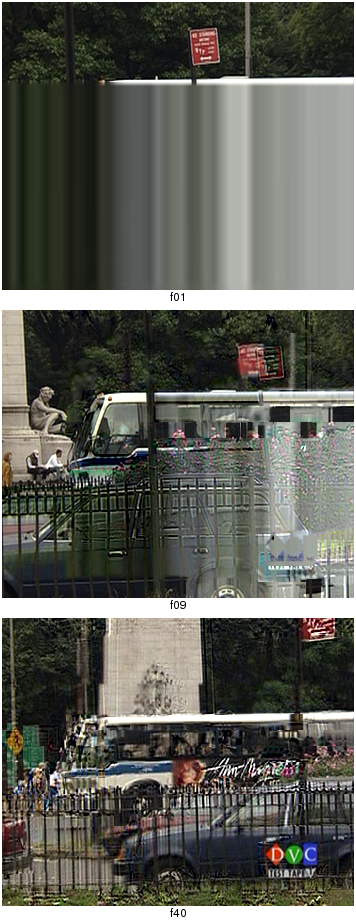
\includegraphics[width=0.9\textwidth]{./imgs/netsim.png}
	\caption{Ilustração do arquivo de configuração de descartes da ferramenta Netsim.}
	\label{fig:netsim}
	\fonte{Autoria Própria.}
\end{figure}

Neste caso, \emph{A} e \emph{C} indicam o número de entidades que atingem seu destino com sucesso e \emph{B} e \emph{D} indicam quantas serão descartadas. 
Sendo assim o streaming de vídeo da Figura \ref{fig:netsim}  teria seus primeiros \emph{A} pacotes intactos, seguidos de \emph{B} perdidos, mais \emph{C} pacotes intactos e ainda \emph{D} perdidos novamente.

\begin{description}
	\item[\texttt{--input}] \hfill \\
		Define o caminho(absoluto ou relativo) e arquivo do vídeo a ser processado pela simulação.
	\item[\texttt{--output}] \hfill \\
		Define o caminho(absoluto ou relativo) e arquivo onde será armazenado o vídeo resultante.
	\item[\texttt{--ts}] \hfill \\
		(Opcional) Se presente, a entidade de descarte considerada é um TS, caso contrário a unidade é um pacote UDP.
	\item[\texttt{--raffle}] \hfill \\
		Indica o caminho(absoluto ou relativo) e arquivo a ser usado como configuração de descartes.
\end{description}


\subsection{Metric}

A ferramenta Metric se trata da implementação de três métricas objetivas, as mesma encontradas na implementação do SASQV:

\begin{itemize}
	\item MSE
	\item PSNR
	\item MSSIM
\end{itemize}

Implementada em C++, também na forma de uma ferramenta \emph{stand-alone}, seu funcionamento é baseado em verificar disparidades entre dois vídeos fornecidos seguindo uma das métricas implementadas e fornecer um resultado numérico. 
Os vídeos a serem comparados devem possuir as mesmas dimensões e número de frames para serem passíveis de comparação. 
A ferramenta Metric pode receber os seguintes parametros:

\begin{description}
	\item[\texttt{--input}] \hfill \\
		Define o caminho(absoluto ou relativo) e arquivo onde um dos vídeos a serem comparados se encontra.
	\item[\texttt{--reference}] \hfill \\
		Define o caminho(absoluto ou relativo) e arquivo onde o segundo vídeo a ser comparado se encontra.
	\item[\texttt{--size}] \hfill \\
		Define as dimensões (em pixels) dos vídeos a serem comparados. Deve ser fornecida no formato 'largura'x'altura'.
	\item[\texttt{--metric}] \hfill \\
		Define qual métrica será utilizada na comparação entre vídeos, sendo uma string entre MSE, PSNR ou MSSIM.
	\item[\texttt{--window}] \hfill \\
		Define qual o tamanho da janela (em pixels) a ser usado se a métrica adotada for MSSIM.
\end{description}

\section{Interface Gráfica}
\subsection{Sessão}
\subsection{Ferramentas}
\subsection{Resultados}
\subsection{Configurações}
\subsection{Ajuda}

\section{Diagramas de Classes}

\section{Diagramas de Sequências}
\section{Considerações}
